%!TEX program = xelatex
\documentclass[xcolor=svgnames,10pt]{beamer}
\usefonttheme[onlymath]{serif}
\usepackage{microtype,enumerate}
\definecolor{dutch}{RGB}{22,147,165}
\definecolor{ral}{RGB}{72,101,145}
\definecolor{ff}{RGB}{255,18,0}
\definecolor{frost}{RGB}{233,237,243}
\definecolor{hel}{RGB}{33,155,237}
% \numberwithin{equation}{section}
\usepackage{bm}
%\setbeamercovered{transparent}
\usecolortheme[RGB={0,81,107}]{structure}  %255,134,24%0,168,82%0,81,107
\setbeamertemplate{caption}[numbered]
\setbeamertemplate{navigation symbols}{}
\useoutertheme{infolines}
\usetheme{Darmstadt}
\setbeamercovered{transparent}
% 修改样式
\setbeamertemplate{blocks}[rounded][shadow=true]
%\setbeamercolor{block title}{fg=frost,bg=dutch}
%%\setbeamercolor{block body}{use=sidebar,fg=black,bg=sidebar.bg!90!blue}
%ce
%\setbeamercolor{block title example}{use=sidebar,fg=sidebar.fg!10!white,bg=dutch}
%\setbeamercolor{block title theorem}
%{use=sidebar,fg=sidebar.fg!10!white,bg=ass}
%%%\setbeamercolor{block body example}{use=sidebar,fg=black,bg=sidebar.bg!90!green}
%%
%\setbeamercolor{block title alerted}{use=sidebar,fg=sidebar.fg!10!white,bg=black!50!red}
%%%\setbeamercolor{block body alerted}{use=sidebar,fg=black,bg=sidebar.bg!90!red}
%\usepackage{times}
%\renewcommand{\rmdefault}{ptm}
\usepackage[T1]{fontenc}
\usepackage{textcomp}
\renewcommand{\rmdefault}{ptm}
\usepackage[scaled=0.92]{helvet}
\usepackage[lite,subscriptcorrection,slantedGreek,nofontinfo]{mtpro2}

\usepackage{fontspec}
\defaultfontfeatures{Mapping=tex-text}
\usepackage{xunicode}
\usepackage{xltxtra}
\usepackage{xeCJK}
\setmainfont{Minion Pro}%
\setsansfont{Myriad Pro}%
\setmonofont{Courier New}
\setCJKmainfont{Adobe Kaiti Std}
%\theoremstyle{example}
%\newtheorem{prop}{Proposition}
\newcounter{prop}
\renewcommand{\theprop}{\arabic{prop}}
\newenvironment{proposition}{\begin{block}{Proposition \stepcounter{prop}\theprop}}{\end{block}}


%\newcounter{Exam}[section]
%\renewcommand{\theExam}{\thesection.\arabic{Exam}}
%\newenvironment{exam}{{\noindent\sc{\color{cyan} Example \stepcounter{Exam}\theExam}}%
%\\[-2ex]{\color{cyan}\rule{\linewidth}{0.8pt}}\color{black}\it\\}{%
%\nopagebreak\\*{\color{cyan}\rule{\linewidth}{0.8pt}}}

\usepackage{indentfirst}
\renewcommand{\figurename}{\textbf{Figure}}
%\renewcommand{\thefigure}{\textbf{\arabic{figure}}}
\newcommand{\figref}[1]{\textbf{Figure}\ref{#1}}
%\numberwithin{figure}{subsection}

\usepackage{hyperref}
\hypersetup{%colorlinks,
						citecolor=red,
						linkcolor={blue},
                    plainpages=false,
                    pdfstartview=FitH,
                    pdfborder={0 0 0},
                    linktocpage,
                    pdfpagemode={FullScreen}
					}

%\pgfdeclareimage{logo}{whu.pdf}%
\title{An Account of Global Factor Trade}
\subtitle{Variants of HOV Model and the Tests}
\author{\mbox{\phantom{Pre. by: Dongsheng} Davis, D.R. and Weinstein, D.E.\phantom{Pre. by: Dongsheng}}\\ \vspace{1ex} Pre. by: Deng Dongsheng}
\institute{ School of Economics, Fudan University}
% \titlegraphic{
\includegraphics[width=0.4\textwidth]{fdu.jpg}}
%\titlegraphic{\pgfuseimage{logo}}%
\usepackage[timeinterval=1]{tdclock}
\date{\today}

\newcommand{\ncite}[1]{{\color{blue}[#1]}}
\begin{document}


\begin{frame}[fragile]
\titlepage{}
\end{frame}
\clearpage

%\begin{frame}
%\tableofcontents
%\end{frame}
\section{Motivation}
\subsection{Motivation}
\begin{frame}[c]\frametitle{Motivation}
\textbf{Why account for factor content of trade?}
\begin{itemize}
    \item  Trace the effects of international influences on relative and absolute factor prices within a country.
    \item It provides a concrete prediction against which to measure how well
our models work.
\end{itemize}
\textbf{Why HOV?}
\begin{itemize}
    \item Sharp predictions for the link btw trade, technology, and endowments.
\end{itemize}
\begin{theorem}[From HOV]
 The net export of factor services will be the difference between a country\rq{}s endowment and the endowment typical in the world for a country of that size.
\end{theorem}

The prediction is \textcolor{orange}{elegant}, \textcolor{orange}{intuitive}, and spectacularly \textcolor{red}{at odds with the data}.

\end{frame}

\section{Theory}
\subsection{Standard HOV}
\begin{frame}[c]\frametitle{Standard HOV}
\textbf{Assumptions}
\begin{itemize}
    \item Identical, CRS production functions for all countries;
    \item Factor and goods mkts are perfectly competitive;
    \item No trade barriers and trade is costless;
    \item Number of goods $\geq$ number of primary factors
    \item Distribution of factors are consistent with the integrated EQ;
    \item Factor prices is equalized $\Rightarrow$ same techniques of production.
    \item Identical and homothetic preferences across countries.
\end{itemize}

\begin{block}{Production and Specification 1}
\begin{align}
\mbf{B}^{c^{\prime}} \mbf{Y}^{c} &= \mbf{V}^{c}\tag{P1}\\
\mbf{B}^{c^{\prime}} \mbf{T}^{c} &= \mbf{B}^{c^{\prime}}(\mbf{Y}^{c}-\mbf{D}^{c}) = \mbf{V}^{c} - s^{c} \mbf{V}^{W} \quad \forall\; c \tag{T1}
\end{align}
\end{block}
\end{frame}

\subsection{A Common Tech Matrix measured with Error}
\begin{frame}[c]\frametitle{A Common Tech Matrix measured with Error}
    Both the true and measured technology matrices are identical across countries (typically U.S. tech). Now, we consider the measurement error, assume that for country $c$ the measured technology matrix is given as
    \begin{equation}
    \ln \mbf{B}^{c}=\ln \mbf{B}^{\mu}+\varepsilon^{c}
    \end{equation}
    $\ln \mbf{B}^{\mu}$ is the natural log of true technology matrix and $\varepsilon$ is a matrix of normal error terms. Then it gives rise to our second set of tests:

\begin{block}{Production and Trade Specification 2:}
\begin{align}
\mbf{B}^{\mu} \mbf{Y}^{c} &= \mbf{V}^{c}\tag{P2}\\
\mbf{B}^{\mu} \mbf{T}^{c} &= \mbf{V}^{c} - s^{c}  \mbf{V}^{W} \quad \forall\; c  \tag{T2}
\end{align}
\end{block}

\end{frame}

\subsection{Hicks-Neutral Technical Differences}
\begin{frame}[c]\frametitle{Hicks-Neutral Technical Differences}
We consider cross-country diffrences in productivity, BLS(1987) and Trefler(1995) use Hicks-neutral technical diffrences as a parimonious way to capture these effects. This can be characterized via \textcolor{orange}{country-specific technology shifts} ${\lambda}^{c}$:
\begin{equation}
\mbf{B}^{c}=\lambda^{c} \mbf{B}^{\lambda} \quad  \forall\; c
\end{equation}

We can express a country\rq{}s endowments in effeciency terms:
\begin{equation}
\mbf{V}^{cE} = \frac{1}{\lambda^{c}} \mbf{V}^{c} \quad \forall\; c
\end{equation}

HOV with effiency units (endowments) becomes:
\begin{block}{Production and Trade Specification 3}
\begin{align}
\mbf{B}^{\lambda} \mbf{Y}^{c} &= \mbf{V}^{cE} \tag{P3} \\
\mbf{B}^{\lambda} \mbf{T}^{c} &= \mbf{V}^{cE} - s^{c} \mbf{V}^{WE} \quad \forall\; c \tag{T3}
\end{align}
\end{block}


\end{frame}

\subsection{DFS model}
\begin{frame}[c]\frametitle{DFS model}
David Dollar et al.(1988) found that capital to labor usage (industry factor usage) is corelated with country capital abundance (factor abundance). Two reasons:
\begin{itemize}
    \item Breakdown in Factor price equalization (NEXT MODEL)
    \item Due to aggregating goods of heterogenous factor content within industry categories.
\end{itemize}

In a two-country DFS model (with continuum of goods), we expect \textcolor{orange}{input usage in correlated with capital abundance for tradables but not for nontradables}. Specification must recognizes that
\begin{itemize}
    \item Tradable industries production varies systematically with country capital abundance.
    \item Absorption should measured with producer country\rq{}s input coeffients.
\end{itemize}
\begin{block}{Production and Trade Specification 4}
\begin{align}
\mbf{B}^{cDFS}\mbf{Y}^{c} &= \mbf{V}^{c} \tag{P4}\\
\mbf{B}^{cDFS}\mbf{Y}^{c} - \Big[\mbf{B}^{cDFS}\mbf{D}^{cc}+\sum_{c^{\prime}\not=c}\mbf{B}^{c^{\prime}DFS} M^{cc^{\prime}}\Big] &=  \mbf{V}^{c} - s^{c} \mbf{V}^{W} \tag{T4}
\end{align}
\end{block}
\end{frame}

\subsection{Helpman no-FPE Model}
\begin{frame}[c]\frametitle{Helpman no-FPE Model}
Consider a economy where the extent of differences in endowments is sufficient that some countries do not share factor price equalization. Model setup:
\begin{equation}
\mbf{B}^{cH} = [\mbf{B}^{cHN}\quad \mbf{B}^{cHT}] \quad \mbf{Y}^{c}=[\mbf{Y}^{cN}\quad\mbf{Y}^{cT}]^{\prime}
\end{equation}
Denote $\mbf{V}^{cN}$ ($\mbf{V}^{cT}$) the resource devoted in country $c$ to production of nontradable (tradable) goods. Namely:
\begin{equation}
\mbf{V}^{cJ}=\mbf{B}^{cHJ}\mbf{Y}^{cJ}\quad  J\in \{N,T\}
\end{equation}

\begin{block}{Production and Trade Specification 5}
\begin{align}
\mbf{B}^{cH}\mbf{Y}^{c} &= \mbf{V}^{c}\tag{P5}\\
\mbf{B}^{cHT}\mbf{Y}^{cT}-\Big[\mbf{B}^{cHT}\mbf{D}^{ccT}+\sum_{c^{\prime}\not = c}\mbf{B}^{c^{\prime}HT}\mbf{M}^{cc^{\prime}}\Big]&=\mbf{V}^{cT}-s^{c} \mbf{V}^{WT}\notag\\
&\hspace{-6ex} = \big[\mbf{V}^{c}-s^{c} \mbf{V}^{W}\big]-\big[\mbf{V}^{cN}-s^{c}\mbf{V}^{WN}\big]
\tag{T5}
\end{align}
\end{block}
\end{frame}

\subsection{Demand, HOV, and Gravity}
\begin{frame}[c]\frametitle{Demand, HOV, and Gravity}
\textbf{Consequence of Frictionless Assumptions:}
\begin{itemize}
    \item Overstates the expected volume of trade
    \item Overstates the opportunities for arbitrage of factor price differences.
\end{itemize}

\textbf{Gravity equation} (use distance as a proxy for costs of trade)
\begin{equation}
\ln (M_{i}^{cc^{\prime}}) = \alpha_{0i}+\alpha_{1i} \ln(s_{i}^{Tc}X_{i}^{c^{\prime}})+ \delta_{i} \ln(d_{cc^{\prime}})+\zeta_{i}^{cc^{\prime}}
\end{equation}
where $X_{i}^{c^{\prime}}$ is gross output in sector $i$ in country $c^{\prime}$, the $\alpha$\rq{}s and $\delta$ are parameters to be estimated. $\hat{\mbf{M}}^{cc^{\prime}}$ are the predicted imports.

\begin{block}{Trade Specification 7:}
\begin{align}
\mbf{B}^{cH}\mbf{Y}^{c} - \Big[\mbf{B}^{cH}\mbf{D}^{cc}+\sum_{c^{\prime}\not=c}\mbf{B}^{c^{\prime}H}\mbf{M}^{cc^{\prime}}\Big]=\mbf{V}^{c}-\Big[\mbf{B}^{cH}\hat{\mbf{D}}^{cc}+\sum_{c^{\prime}\not = c}\mbf{B}^{c^{\prime}H}\hat{\mbf{M}}^{cc^{\prime}}\Big]\tag{T7}
\end{align}
\end{block}
Set demand for domestically produced goods($\hat{\mbf{D}}^{cc}$) = total demand - total imports from gravity equation($\sum_{c^{\prime}\not = c}\hat{\mbf{M}}^{cc^{\prime}} $).
\end{frame}

\begin{frame}[c]\frametitle{Summary of Specifications}
\begin{center}
\text{Summary of Specifications (Grouping)}
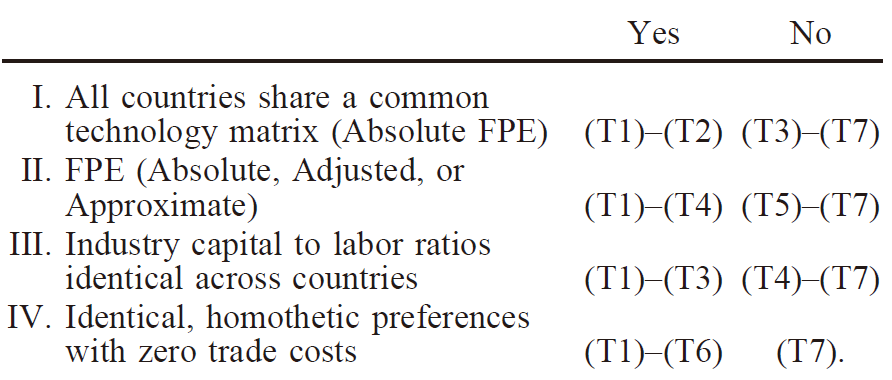
\includegraphics[width=0.6\textwidth]{sum.png}
\end{center}
\end{frame}

\section{Data Sources and Issues}
\subsection{Data Sources and Issues}
\begin{frame}[c]\frametitle{Data}
\textbf{Data Sources}
\begin{itemize}
    \item OECD countries (10 con*34 ind): technology, net output, endowments, absorption and trade data.
    \begin{itemize}
    \item The Organization for Economic Cooperation and Development\rq{}s Input-Output Database [OECD (1995)]
    \item OECD\rq{}s International Sectoral Database $\Rightarrow$ endowment data
    \item The OECD\rq{}s STAN Database $\Rightarrow$ input requirements
    \end{itemize}
    \item ROW (Rest of World):
    \begin{itemize}
    \item Capital: Robert Summers and Alan W. Heston (1997) Database
    \item Labor: International Labor Organization
    \item Gross output: United Nation\rq{}s Industrial Statistics Yearbook
    \end{itemize}
    \item Bilateral trade flows: Draw from Robert C. Feenstra et al.(1997)
    \item Bilateral distance: Shang-Jin Wei(1996)
\end{itemize}

For more info. about data and data manipulation, please ref the \textcolor{orange}{Data Appendix}.
\end{frame}

\section{Estimation}
\subsection{Estimating Technology}
\begin{frame}[allowframebreaks]\frametitle{Estimating Technology}
\begin{enumerate}
\item For indentical technology (P1): \\
$\mbf{B}^{c}=\mbf{B}^{c^{\prime}}$, We reject this restriction by inspection.
\item For measurement error model (P2):
\begin{equation}
\ln B_{fi}^{c} = \beta_{fi} + \varepsilon_{fi}^{c} \tag{$\hat{\text{P}}2$}
\end{equation}
$\beta_{fi}$ are parameters to be estimated corresponding to the log of common factor input requirement for factor $f$ in sector $i$.
\item For Hicks-neutral technical differences (P3):
\begin{equation}
\ln B_{fi}^{c} = \theta^{c}+\beta_{fi}^{c}+\psi_{fi}^{c} \tag{$\hat{\text{P}}3$}
\end{equation}
where $e^{\theta^{c}} = \lambda^{c}$. Normalization for $\theta^{c}$, set $\theta^{US}=0 (\lambda^{US}=1)$.
\item For DFS model (P4):
\begin{equation}
\ln B_{fi}^{c} = \theta^{c} + \beta_{fi}+\gamma_{f}^{T}\ln\Big(\frac{K^{c}}{L^{c}}\Big) TRAD_{i} + \phi_{fi}^{c} \tag{$\hat{\text{P}}4$}
\end{equation}
$TRAD_{i}$ is dummy variable that takes value of one if the sector is tradable.
\item For FPE breaks down model (P5):
\begin{equation}
\ln B_{fi}^{c} = \theta^{c} + \beta_{fi}+\gamma_{f}^{T}\ln\Big(\frac{K^{c}}{L^{c}}\Big) TRAD_{i}  + \gamma_{f}^{NT}\ln\Big(\frac{K^{c}}{L^{c}}\Big) NT_{i} + \phi_{fi}^{c} \tag{$\hat{\text{P}}5$}
\end{equation}
\item More Genernal Specification:
\begin{equation}
\ln B_{fi}^{c} = \theta^{c} + \beta_{fi}+\gamma_{fi}\ln\Big(\frac{K^{c}}{L^{c}}\Big)  + \phi_{fi}^{c} \tag{$\hat{\text{P}}5^{\prime}$}
\end{equation}
\textbf{method:} In each specification, we have 68 equations, SUR will used up the degress of freedom. We estimated these equations as \textcolor{orange}{a system of SUR with cross-equation restrictions but imposed a diagonal variance-covariance matrix on the residuals}.
\end{enumerate}
\end{frame}
\subsection{Technological Variation}
\begin{frame}[plain]
\centering
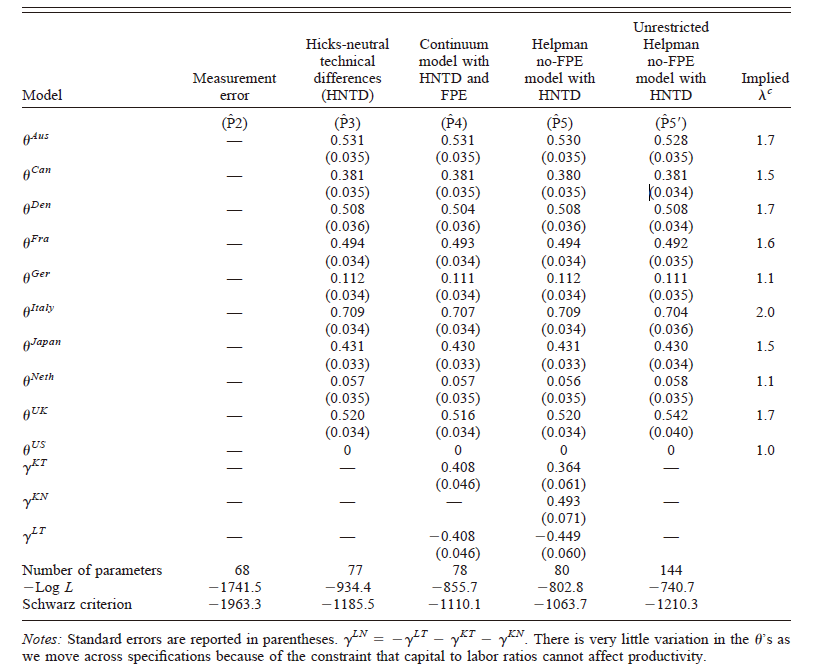
\includegraphics[width=0.85\textwidth]{tech.png}
\end{frame}

\subsection{Estimating Demand}
\begin{frame}[c]\frametitle{Estimating Demand}
We use a gravity model as the basis for our demand predictions in specification (T7),
\begin{equation}
\ln (M_{i}^{cc^{\prime}}) = \alpha_{0i}+\alpha_{1i} \ln(s_{i}^{Tc}X_{i}^{c^{\prime}})+ \delta_{i} \ln(d_{cc^{\prime}})+\zeta_{i}^{cc^{\prime}}
\end{equation}
\begin{itemize}
    \item zero-trade-cost case: $\alpha_{0i}=\delta_{i}=0$
    \item result: $\alpha_{1i}$ close to 1, $\delta_{i}$ is significant and negative in all sectors, $\Rightarrow$ statistical rejection the hypothesis of costless trade.
\end{itemize}

\textbf{Problem:} In some sectors we found large systematic errors in predicting trade with the ROW. This may be the result of mis-measurement of distance or the fact that the true ROW is some multiple of our sample of countries.\\
\textbf{Solution:} Add dummy variables corresponding the country importing country being the ROW.
\end{frame}

\section{Production and Trade Tests}
\subsection{Key Specifications}
\begin{frame}[c]{Key Specifications}
\centering
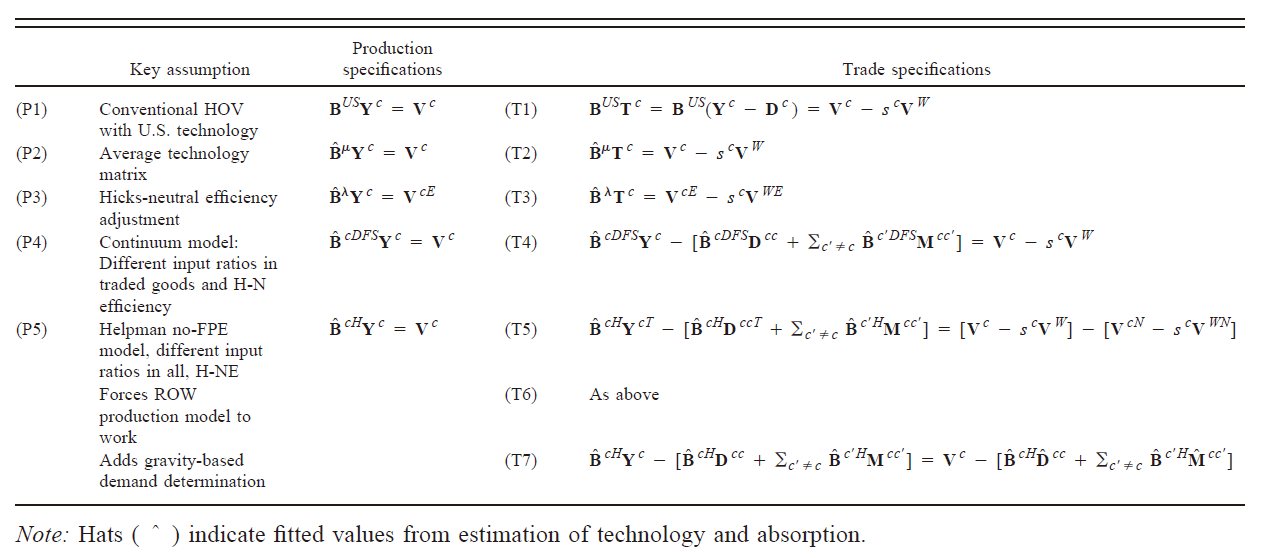
\includegraphics[width=\textwidth]{spec.png}
\end{frame}

\subsection{Production and Trade Tests}
\begin{frame}[c]\frametitle{Production and Trade Tests}
\begin{itemize}
\item Production tests:
    \begin{itemize}
    \item Slope Test: Regress MFCP on PFCP \quad ex. \quad \ $\mbf{B}^{f}\mbf{Y}^{c} \text{\;on\;} \mbf{V}^{fc}$ \\
    \item Median Error Test: ex. $|\mbf{B}_{f}^{US}\mbf{Y}^{c}-\mbf{V}_{f}^{c}|/\mbf{V}_{f}^{c}$.
    \end{itemize}
\item Trade tests:
    \begin{itemize}
        \item Sign Test: $\text{sign}(MFCT) = \text{sign}(PFCT)$?
        \item Slope Test: Regress MFCT on PFCT.
        \item Variance Ratio Test: $Var(MFCT)/Var(PFCT)$
    \end{itemize}
\end{itemize}
One indicator of ``missing trade'' is when the variance ratio is close to zero, whereas if the model fit perfectly, the variance ratio would be unity.
\end{frame}

\subsection{Production and Trade Results}
\begin{frame}[c]\frametitle{Production and Trade Results}
\centering
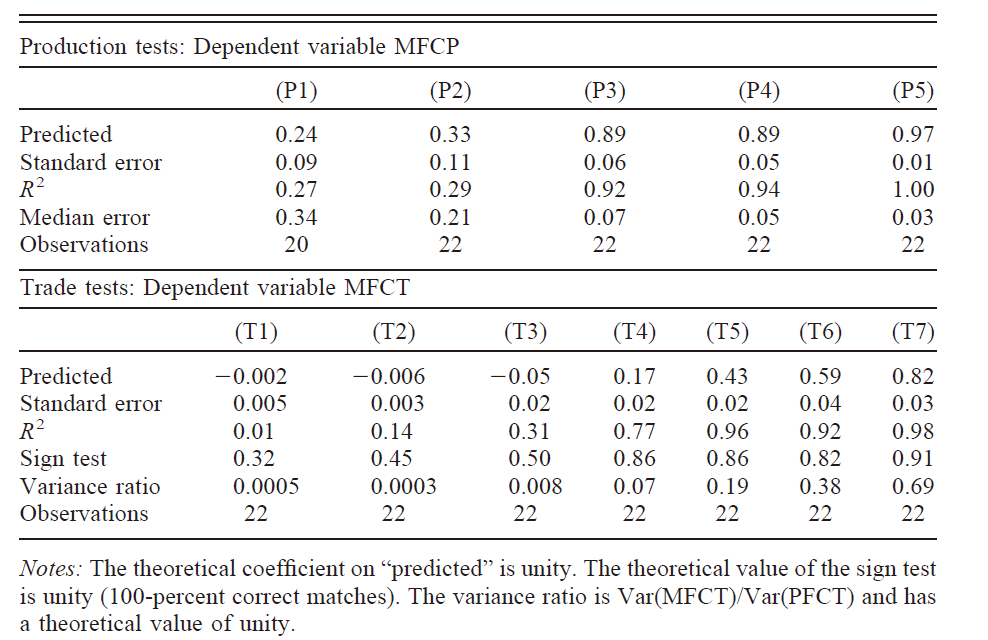
\includegraphics[width=0.95\textwidth]{resu.png}
\end{frame}

\begin{frame}[c]\frametitle{Simple HOV Model}
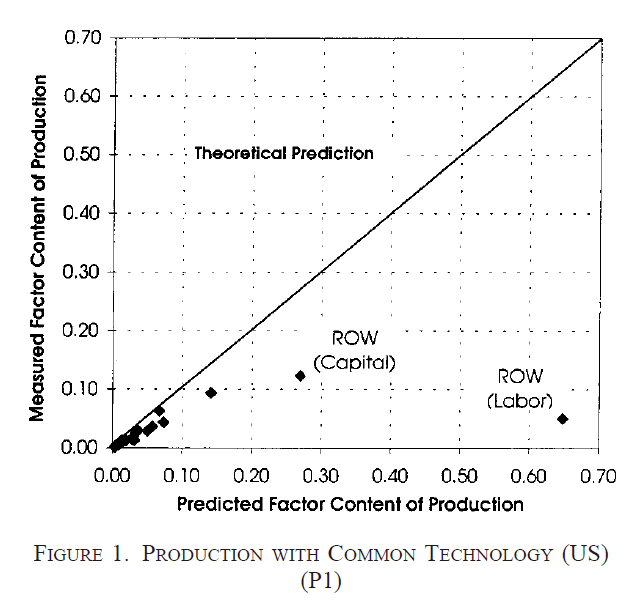
\includegraphics[width=0.5\textwidth]{P1.png}
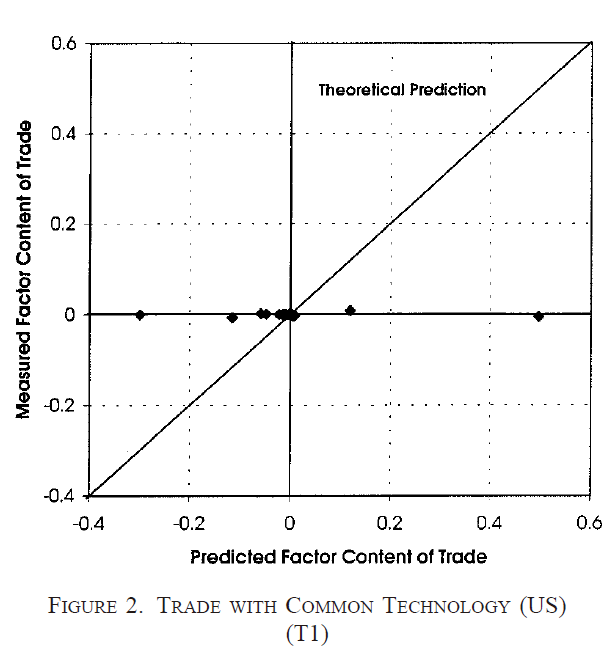
\includegraphics[width=0.5\textwidth]{T1.png}
\end{frame}

\begin{frame}[c]\frametitle{Failure of FPE and Factor Usage in Nontraded Production}
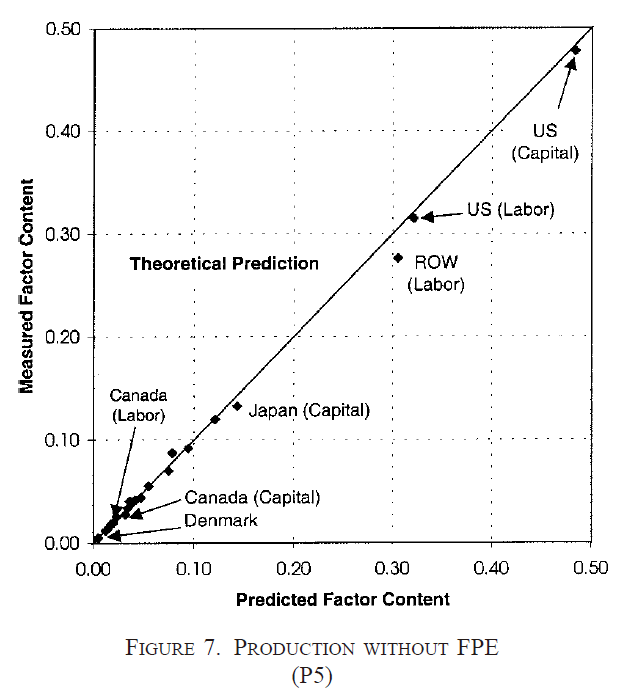
\includegraphics[width=0.5\textwidth]{P5.png}
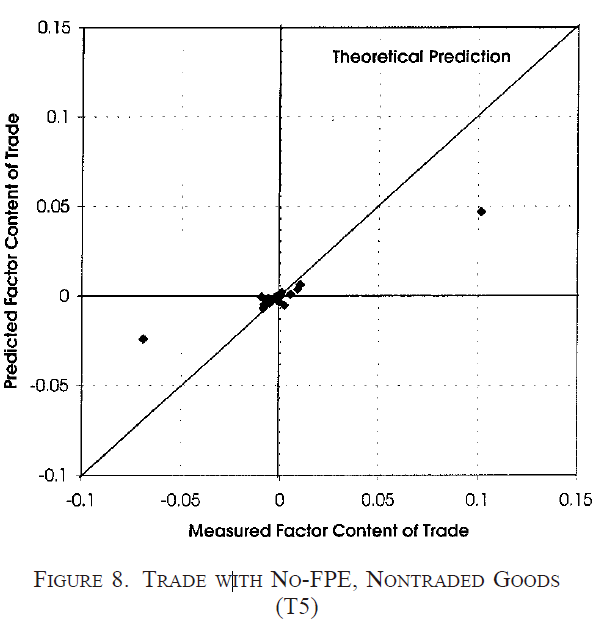
\includegraphics[width=0.5\textwidth]{T5.png}
\end{frame}
\begin{frame}[c]\frametitle{Corrections on ROW Technology V.S. Gravity Demand HOV}
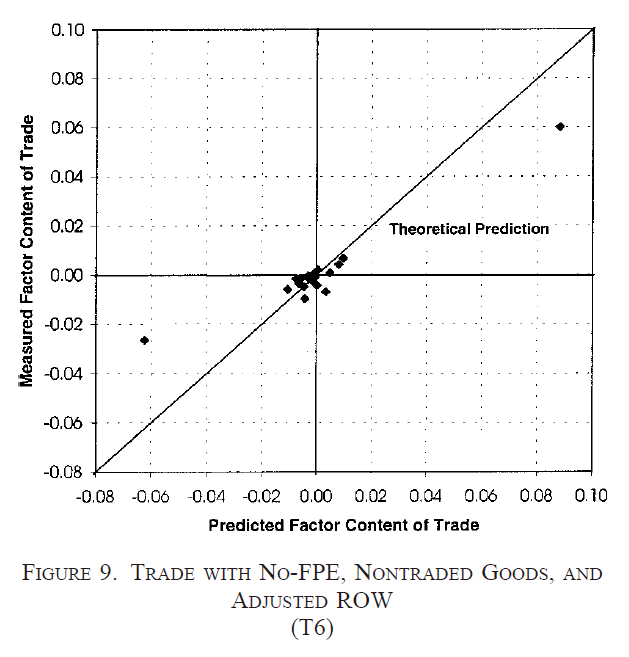
\includegraphics[width=0.5\textwidth]{T6.png}
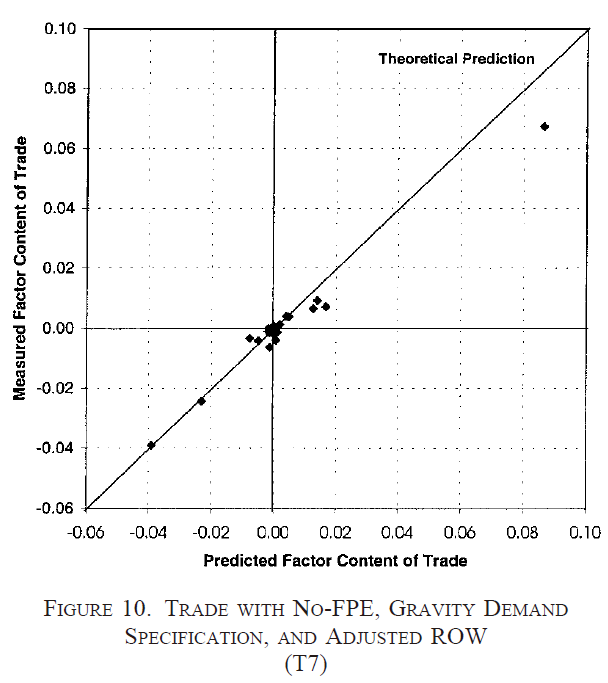
\includegraphics[width=0.5\textwidth]{T7.png}
\end{frame}

\section{Conclusion}
\subsection{Conclusion}
\begin{frame}[c]\frametitle{Conclusion}

\begin{itemize}
\item The study shows that variants of HOV model that permits technical differences, a breakdown in factor price equalization, the existence of nontraded goods, and cost of trade can bring HOV theory and data into congruence.
\item  Conditional on these amendments, countries export their abundant factors and they do so in approximately the right magnitudes.
\item  It is a plausible and simple set of departures from the conventional model allows us to so accurately match the international data.
\end{itemize}
\end{frame}

\end{document}
